\bta{平抛运动}

\begin{enumerate}[leftmargin=0em]
\renewcommand{\labelenumi}{\arabic{enumi}.}
% A(\Alph) a(\alph) I(\Roman) i(\roman) 1(\arabic)
%设定全局标号series=example	%引用全局变量resume=example
%[topsep=-0.3em,parsep=-0.3em,itemsep=-0.3em,partopsep=-0.3em]
%可使用leftmargin调整列表环境左边的空白长度 [leftmargin=0em]
\item
\exwhere{$ 2019 $年物理全国\lmd{2}卷}
如图($ a $),在跳台滑雪比赛中,运动员在空中滑翔时身体的姿态会影响其下落的速度和滑翔的距离。某运动员先后两次从同一跳台起跳,每次都从离开跳台开始计时,用$ v $表示他在竖直方向的速度,其$ v-t $图像如图($ b $)所示,$ t_{1} $和$ t_{2} $是他落在倾斜雪道上的时刻。则 \xzanswer{BD} 
\begin{figure}[h!]
\centering
\includesvg[width=0.23\linewidth]{picture/svg/543}
\end{figure}


\fourchoices
{第二次滑翔过程中在竖直方向上的位移比第一次的小}
{第二次滑翔过程中在水平方向上的位移比第一次的大}
{第一次滑翔过程中在竖直方向上的平均加速度比第一次的大}
{竖直方向速度大小为$ v_{1} $时,第二次滑翔在竖直方向上所受阻力比第一次的大}





\item 
\exwhere{$ 2017 $年新课标 \lmd{1} 卷}
发球机从同一高度向正前方依次水平射出两个速度不同的乒乓球(忽略空气的影响)。速度较大的球越过球网,速度较小的球没有越过球网,其原因是 \xzanswer{C} 

\fourchoices
{速度较小的球下降相同距离所用的时间较多}
{速度较小的球在下降相同距离时在竖直方向上的速度较大}
{速度较大的球通过同一水平距离所用的时间较少}
{速度较大的球在相同时间间隔内下降的距离较大}



\item 
\exwhere{$ 2017 $年新课标$ \lmd{2} $卷}
如图,半圆形光滑轨道固定在水平地面上,半圆的直径与地面垂直,一小物快以速度从轨道下端滑入轨道,并从轨道上端水平飞出,小物快落地点到轨道下端的距离与轨道半径有关,此距离最大时,对应的轨道半径为(重力加速度为$ g $) \xzanswer{B} 
\begin{figure}[h!]
\centering
\includesvg[width=0.23\linewidth]{picture/svg/544}
\end{figure}

\fourchoices
{$ \frac { v ^ { 2 } } { 16 g } $}
{$ \frac { v ^ { 2 } } { 8 g } $}
{$ \frac { v ^ { 2 } } { 4 g } $}
{$ \frac { v ^ { 2 } } { 2 g } $}



\item 
\exwhere{$ 2017 $年江苏卷}
如图所示,$ A $、$ B $两小球从相同高度同时水平抛出,经过时间$ t $在空中相遇,若两球的抛出速度都变为原来的$ 2 $倍,则两球从抛出到相遇经过的时间为 \xzanswer{C} 
\begin{figure}[h!]
\centering
\includesvg[width=0.23\linewidth]{picture/svg/545}
\end{figure}

\fourchoices
{$ t $}
{$ \frac{\sqrt{2}}{2}t $}
{$ \frac{t}{2} $}
{$ \frac{t}{4} $}




\item 
\exwhere{$ 2017 $年浙江选考卷}
图中给出某一通关游戏的示意图,安装在轨道$ AB $上可上下移动的弹射器,能水平射出速度大小可调节的弹丸,弹丸射出口在$ B $点的正上方,竖直面内的半圆弧$ BCD $的半径为$ R=2.0m $,直径$ BD $水平且与轨道$ AB $处在同一竖直平面内,小孔$ P $和圆心$ O $连线与水平方向夹角为$ 37 ^{\circ} $,游戏要求弹丸垂直于$ P $点圆弧切线方向射入小孔$ P $就能进入下一关。为了能通关,弹射器离$ B $点的高度和弹丸射出的初速度分别是(不计空气阻力) \xzanswer{A} 
\begin{figure}[h!]
\centering
\includesvg[width=0.23\linewidth]{picture/svg/546}
\end{figure}

\fourchoices
{$ 0.15\ \mathrm { m } , 4 \sqrt { 3 }\ \mathrm { m } / \mathrm { s } $}
{$ 1.50\ \mathrm { m } , 4 \sqrt { 3 }\ \mathrm { m } / \mathrm { s } $}
{$ 0.15\ \mathrm { m } , 2 \sqrt { 6 }\ \mathrm { m } / \mathrm { s } $}
{$ 1.50\ \mathrm { m } , 2 \sqrt { 6 }\ \mathrm { m } / \mathrm { s } $}




\item 
\exwhere{$ 2013 $年上海卷}
如图,轰炸机沿水平方向匀速飞行,到达山坡底端正上方时释放一颗炸弹,并垂直击中山坡上的目标$ A $。已知$ A $点高度为$ h $,山坡倾角为$ \theta $,由此可算出 \xzanswer{ABC} 
\begin{figure}[h!]
\centering
\includesvg[width=0.23\linewidth]{picture/svg/548}
\end{figure}

\fourchoices
{轰炸机的飞行高度}
{轰炸机的飞行速度}
{炸弹的飞行时间}
{炸弹投出时的动能}


\item 
\exwhere{$ 2012 $年理综新课标卷}
如图,$ x $轴在水平地面内,$ y $轴沿竖直方向。图中画出了从$ y $轴上沿$ x $轴正向抛出的三个小球$ a $、$ b $和$ c $的运动轨迹,其中$ b $和$ c $是从同一点抛出的,不计空气阻力,则 \xzanswer{BD} 
\begin{figure}[h!]
\centering
\includesvg[width=0.23\linewidth]{picture/svg/549}
\end{figure}

\fourchoices
{$ a $的飞行时间比$ b $的长}
{$ b $和$ c $的飞行时间相同}
{$ a $的水平速度比$ b $的小}
{$ b $的初速度比$ c $的大}


\item 
\exwhere{$ 2012 $年物理江苏卷}
如图所示,相距$ l $ 的两小球$ A $、$ B $位于同一高度$ h(l,h $均为定值). 将$ A $向$ B $水平抛出的同时,$ B $自由下落 $. A $、$ B $与地面碰撞前后,水平分速度不变,竖直分速度大小不变、方向相反. 不计空气阻力及小球与地面碰撞的时间,则 \xzanswer{AD} 
\begin{figure}[h!]
\centering
\includesvg[width=0.23\linewidth]{picture/svg/550}
\end{figure}





\fourchoices
{$ A $、$ B $在第一次落地前能否相碰,取决于$ A $的初速度}
{$ $ $ A $、$ B $在第一次落地前若不碰,之后就不会相碰}
{$ A $、$ B $不可能运动到最高处相碰}
{$ A $、$ B $一定能相碰}




\item 
\exwhere{$ 2012 $年理综福建卷}
如图,置于圆形水平转台边缘的小物块随转台加速转动,当转速达到某一数值时,物块恰好滑离转台开始做平抛运动。现测得转台半径$ R=0.5 $ $ m $,离水平地面的高度$ H=0.8m $,物块平抛落地过程水平位移的大小$ s=0.4m $。设物块所受的最大静摩擦力等于滑动摩擦力,取重力加速度$ g=10 \ m/s^{2} $ 求:
\begin{enumerate}
\renewcommand{\labelenumi}{\arabic{enumi}.}
% A(\Alph) a(\alph) I(\Roman) i(\roman) 1(\arabic)
%设定全局标号series=example	%引用全局变量resume=example
%[topsep=-0.3em,parsep=-0.3em,itemsep=-0.3em,partopsep=-0.3em]
%可使用leftmargin调整列表环境左边的空白长度 [leftmargin=0em]
\item
物块做平抛运动的初速度大小$ v_{0} $;
\item 
物块与转台间的动摩擦因数$ \mu $。

\end{enumerate}
\begin{figure}[h!]
\flushright
\includesvg[width=0.25\linewidth]{picture/svg/551}
\end{figure}


\banswer{
\begin{enumerate}
\renewcommand{\labelenumi}{\arabic{enumi}.}
% A(\Alph) a(\alph) I(\Roman) i(\roman) 1(\arabic)
%设定全局标号series=example	%引用全局变量resume=example
%[topsep=-0.3em,parsep=-0.3em,itemsep=-0.3em,partopsep=-0.3em]
%可使用leftmargin调整列表环境左边的空白长度 [leftmargin=0em]
\item
$ 1 \ m/s $
\item 
$ \mu=0.2 $


\end{enumerate}


}



\item 
\exwhere{$ 2012 $年物理上海卷}
如图,斜面上$ a $、$ b $、$ c $三点等距,小球从$ a $点正上方$ O $点抛出,做初速为$ v_{0} $的平抛运动,恰落在$ b $点。若小球初速变为$ v $,其落点位于$ c $,则 \xzanswer{A} 
\begin{figure}[h!]
\centering
\includesvg[width=0.23\linewidth]{picture/svg/552}
\end{figure}


\fourchoices
{$ v_{0} < $ $ v $ $ <2 v_{0} $}
{$ v=2 v_{0} $}
{$ 2 v_{0} < $ $ v <3 v_{0} $ }
{$ v>3 v_{0} $}



\item 
\exwhere{$ 2016 $年江苏卷}
有$ A $、$ B $两小球,$ B $的质量为$ A $的两倍.现将它们以相同速率沿同一方向抛出,不计空气阻力。图中①为$ A $的运动轨迹,则$ B $的运动轨迹是 \xzanswer{A} 
\begin{figure}[h!]
\centering
\includesvg[width=0.23\linewidth]{picture/svg/553}
\end{figure}

\fourchoices
{①}
{②}
{③}
{④}


\item 
\exwhere{$ 2016 $年海南卷}
在地面上方某一点将一小球以一定的初速度沿水平方向抛出,不计空气阻力,则小球在随后的运动中 \xzanswer{B} 

\fourchoices
{速度和加速度的方向都在不断变化}
{速度与加速度方向之间的夹角一直减小}
{在相等的时间间隔内,速率的该变量相等}
{在相等的时间间隔内,动能的改变量相等}



\item 
\exwhere{$ 2018 $年江苏卷}
某弹射管每次弹出的小球速度相等.在沿光滑竖直轨道自由下落过程中,该弹射管保持水平,先后弹出两只小球.忽略空气阻力,两只小球落到水平地面的 \xzanswer{B} 

\fourchoices
{时刻相同,地点相同}
{时刻相同,地点不同}
{时刻不同,地点相同}
{时刻不同,地点不同}


\item 
\exwhere{$ 2018 $年全国 \lmd{3}卷}
在一斜面顶端,将甲、乙两个小球分别以$ v $和$ \frac{v}{2} $的速度沿同一方向水平抛出,两球都落在该斜面上。甲球落至斜面时的速率是乙球落至斜面时速率的 \xzanswer{A} 

\fourchoices
{$ 2 $倍}
{$ 4 $倍	}
{$ 6 $倍}
{$ 8 $倍}


\item 
\exwhere{$ 2011 $年理综广东卷}
如图所示,在网球的网前截击练习中,若练习者在球网正上方距地面$ H $处,将球以速度$ v $沿垂直球网的方向击出,球刚好落在底线上。已知底线到网的距离为$ L $,重力加速度取$ g $,将球的运动视作平抛运动,下列表述正确的是 \xzanswer{AB} 
\begin{figure}[h!]
\centering
\includesvg[width=0.23\linewidth]{picture/svg/554}
\end{figure}

\fourchoices
{球的速度$ v $等于$L \sqrt { \frac { g } { 2 H } }$}
{球从击出至落地所用时间为$\sqrt { \frac { 2 H } { g } }$}
{球从击球点至落地点的位移等于$ L $}
{球从击球点至落地点的位移与球的质量有关}




\item 
\exwhere{$ 2011 $年海南卷}
如图,水平地面上有一个坑,其竖直截面为半圆。$ ab $为沿水平方向的直径。若在$ a $点以初速度$ v_{0} $沿$ ab $方向抛出一小球,小球会击中坑壁上的$ c $点。已知$ c $点与水平地面的距离为圆半径的一半,求圆的半径。
\begin{figure}[h!]
\flushright
\includesvg[width=0.25\linewidth]{picture/svg/555}
\end{figure}

\banswer{
$r = \frac { 4 ( 7 - 4 \sqrt { 3 } ) } { g } v _ { 0 } ^ { 2 }$
}


\item 
\exwhere{$ 2014 $年理综天津卷}
半径为$ R $的水平圆盘绕过圆心$ O $的竖直轴匀速转动,$ A $为圆盘边缘上一点.点$ O $的正上方有一个可视为质点的小球以初速度$ v $水平抛出时,半径$ OA $方向恰好与$ v $的方向相同,如图所示.若小球与圆盘只碰一次,且落在$ A $点,重力加速度为$ g $,则小球抛出时距$ O $的高度$ h= $\tk{$\frac { g R ^ { 2 } } { 2 v ^ { 2 } }$},圆盘转动的角速度大小$ \omega = $\tk{$\frac { 2 \pi n v } { R } \left( n \in N ^ { * } \right)$}. 
\begin{figure}[h!]
\centering
\includesvg[width=0.23\linewidth]{picture/svg/556}
\end{figure}



\item 
\exwhere{$ 2013 $年北京卷}
在实验操作前应该对实验进行适当的分析。研究平抛运动的实验装置示意如图。小球每次都从斜槽的同一位置无初速度释放,并从斜槽末端水平飞出。改变水平板的高度,就改变了小球在板上落点的位置,从而可描绘出小球的运动轨迹。某同学设想小球先后三次做平抛,将水平板依次放在如图$ 1 $、$ 2 $、$ 3 $的位置,且$ 1 $与$ 2 $的间距等于$ 2 $与$ 3 $的间距。若三次实验中,小球从抛出点到落点的水平位移依次为$ x_{1} $、$ x_{2} $、$ x_{3} $,机械能的变化量依次为$ \Delta E_{1} $、$ \Delta E_{2} $、$ \Delta E_3 $,忽略空气阻力的影响,下面分析正确的是 \xzanswer{B} 
\begin{figure}[h!]
\centering
\includesvg[width=0.23\linewidth]{picture/svg/557}
\end{figure}

\fourchoices
{$ x_{2} - x_{1} =x_3- x_{2} $,$ \Delta E_{1} = \Delta E_{2} = \Delta E_3 $}
{$ x_{2} - x_{1} >x_3- x_{2} $,$ \Delta E_{1} = \Delta E_{2} = \Delta E_3 $}
{$ x_{2} - x_{1} >x_3- x_{2} $,$ \Delta E_{1} < \Delta E_{2} < \Delta E_3 $}
{$ x_{2} - x_{1} <x_3- x_{2} $,$ \Delta E_{1} < \Delta E_{2} < \Delta E_3 $}



\item 
\exwhere{$ 2013 $年江苏卷}
如图所示,从地面上同一位置抛出两小球$ A $、$ B $,分别落在地面上的$ M $、$ N $ 点,两球运动的最大高度相同. 空气阻力不计,则 \xzanswer{CD} 
\begin{figure}[h!]
\centering
\includesvg[width=0.23\linewidth]{picture/svg/558}
\end{figure}





\fourchoices
{$ B $ 的加速度比$ A $ 的大}
{$ B $ 的飞行时间比$ A $ 的长}
{$ B $ 在最高点的速度比$ A $ 在最高点的大}
{$ B $ 在落地时的速度比$ A $ 在落地时的大}


\item 
\exwhere{$ 2014 $年物理上海卷}
如图,宽为$ L $的竖直障碍物上开有间距$ d=0.6\ m $的矩形孔,其下沿离地高$ h=1.2m $,离地高$ H=2m $的质点与障碍物相距$ x $。在障碍物以$ v_{0} =4 \ m/s $匀速向左运动的同时,质点自由下落。为使质点能穿过该孔,$ L $的最大值为 \tk{0.8} $ m $;若$ L $ $ =0.6m $, $ x $的取值范围是 \tk{$ 0.8m \leq x \leq 1m $} $ m $。(取$ g=10 \ m/s^{2} ) $
\begin{figure}[h!]
\centering
\includesvg[width=0.23\linewidth]{picture/svg/559}
\end{figure}



\item 
\exwhere{$ 2014 $年理综浙江卷}
如图所示,装甲车在水平地面上以速度$ v_{0} =20 \ m/s $沿直线前进,车上机枪的枪管水平,距地面高为$ h=1.8\ m $。在车正前方竖直一块高为两米的长方形靶,其底边与地面接触。枪口与靶距离为$ L $时,机枪手正对靶射出第一发子弹,子弹相对于枪口的初速度为$ v=800 \ m/s $。在子弹射出的同时,装甲车开始匀减速运动,行进$ s=90\ m $后停下。装甲车停下后,机枪手以相同方式射出第二发子弹。(不计空气阻力,子弹看成质点,重力加速度$ g=10 \ m/s^{2} $).
\begin{enumerate}
\renewcommand{\labelenumi}{\arabic{enumi}.}
% A(\Alph) a(\alph) I(\Roman) i(\roman) 1(\arabic)
%设定全局标号series=example	%引用全局变量resume=example
%[topsep=-0.3em,parsep=-0.3em,itemsep=-0.3em,partopsep=-0.3em]
%可使用leftmargin调整列表环境左边的空白长度 [leftmargin=0em]
\item
求装甲车匀减速运动时的加速度大小;
\item 
当$ L=410\ m $时,求第一发子弹的弹孔离地的高度,并计算靶上两个弹孔之间的距离;
\item 
若靶上只有一个弹孔,求$ L $的范围。

\end{enumerate}
\begin{figure}[h!]
\flushright
\includesvg[width=0.25\linewidth]{picture/svg/560}
\end{figure}


\banswer{
\begin{enumerate}
\renewcommand{\labelenumi}{\arabic{enumi}.}
% A(\Alph) a(\alph) I(\Roman) i(\roman) 1(\arabic)
%设定全局标号series=example	%引用全局变量resume=example
%[topsep=-0.3em,parsep=-0.3em,itemsep=-0.3em,partopsep=-0.3em]
%可使用leftmargin调整列表环境左边的空白长度 [leftmargin=0em]
\item
$a = \frac { v _ { 0 } ^ { 2 } } { 2 s } = \frac { 20 } { 9 } \mathrm { m } / \mathrm { s } ^ { 2 }$

\item 
第一发子弹弹孔离地高度$h _ { 1 } = h - \frac { 1 } { 2 } g t _ { 1 } ^ { 2 } = 0.55 \mathrm { m }$ \qquad 两弹孔之间的距离$\Delta h = h _ { 2 } - h _ { 1 } = 0.45 \mathrm { m }$
\item 
$492 \mathrm { m } < L \leq 570 \mathrm { m }$

\end{enumerate}


}




\item 
\exwhere{$ 2015 $年理综新课标 \lmd{1} 卷}
一带有乒乓球发射机的乒乓球台如图所示。水平台面的长和宽分别为$ L_{1} $和$ L_{2} $,中间球网高度为$ h $.发射机安装于台面左侧边缘的中点,能以不同速率向右侧不同方向水平发射乒乓球,发射点距台面高度为$ 3 h $。不计空气的作用,重力加速度大小为$ g $。若乒乓球的发射速率$ v $在某范围内,通过选择合适的方向,就能使乒乓球落到球网右侧台面上,则$ v $的最大取值范围是 \xzanswer{D} 
\begin{figure}[h!]
\centering
\includesvg[width=0.23\linewidth]{picture/svg/561}
\end{figure}

\fourchoices
{$\frac { L _ { 1 } } { 2 } \sqrt { \frac { g } { 6 h } } < v < L _ { 1 } \sqrt { \frac { g } { 6 h } }$}
{$\frac { L _ { 1 } } { 4 } \sqrt { \frac { g } { h } } < v < \sqrt { \frac { \left( 4 L _ { 1 } ^ { 2 } + L _ { 2 } ^ { 2 } \right) g } { 6 h } }$}
{$\quad \frac { L _ { 1 } } { 2 } \sqrt { \frac { g } { 6 h } } < v < \frac { 1 } { 2 } \sqrt { \frac { \left( 4 L _ { 1 } ^ { 2 } + L _ { 2 } ^ { 2 } \right) g } { 6 h } }$}
{$\quad \frac { L _ { 1 } } { 4 } \sqrt { \frac { g } { h } } < v < \frac { 1 } { 2 } \sqrt { \frac { \left( 4 L _ { 1 } ^ { 2 } + L _ { 2 } ^ { 2 } \right) g } { 6 h } }$}

\item 
\exwhere{$ 2015 $年理综重庆卷}
同学们参照伽利略时期演示平抛运动的方法制作了如题$ 8 $图所示的实验装置。图中水平放置的底板上竖直地固定有$ M $板和$ N $板.$ M $ 板上部有一半径为$ R $的$ \frac{ 1 }{ 4 } $圆弧形的粗糙轨道,$ P $为最高点,$ Q $为最低点,$ Q $点处的切线水平,距底板高为$ H $。$ N $板上固定有三个圆环。将质量为$ m $的小球从$ P $处静止释放,小球运动至$ Q $飞出后无阻碍地通过各圆环中心,落到底板上距$ Q $水平距离为$ L $处。不考虑空气阻力,重力加速度为$ g $。求:
\begin{enumerate}
\renewcommand{\labelenumi}{\arabic{enumi}.}
% A(\Alph) a(\alph) I(\Roman) i(\roman) 1(\arabic)
%设定全局标号series=example	%引用全局变量resume=example
%[topsep=-0.3em,parsep=-0.3em,itemsep=-0.3em,partopsep=-0.3em]
%可使用leftmargin调整列表环境左边的空白长度 [leftmargin=0em]
\item
距$ Q $水平距离为的圆环中心到底板的高度;
\item 
小球运动到$ Q $点时速度的大小以及对轨道压力的大小和方向;
\item 
摩擦力对小球做的功.

\end{enumerate}
\begin{figure}[h!]
\centering
\includesvg[width=0.23\linewidth]{picture/svg/562}
\end{figure}


\banswer{
\begin{enumerate}
\renewcommand{\labelenumi}{\arabic{enumi}.}
% A(\Alph) a(\alph) I(\Roman) i(\roman) 1(\arabic)
%设定全局标号series=example	%引用全局变量resume=example
%[topsep=-0.3em,parsep=-0.3em,itemsep=-0.3em,partopsep=-0.3em]
%可使用leftmargin调整列表环境左边的空白长度 [leftmargin=0em]
\item
$ \frac{ 3 }{ 4 } H $
\item 
速度的大小为$L \sqrt { \frac { g } { 2 H } }$ ,压力的大小$m g + \frac { m g L ^ { 2 } } { 2 H R }$,方向竖直向下 ;
\item 
摩擦力对小球作功$\frac { m g L ^ { 2 } } { 4 H } - m g R$

\end{enumerate}


}


\item 
\exwhere{$ 2015 $年理综浙江卷}
如图所示为足球球门,球门宽为$ L $。一个球员在球门中心正前方距离球门$ s $处高高跃起,将足球顶入球门的左下方死角(图中$ P $点)。球员顶球点的高度为$ h $。足球做平抛运动(足球可看做质点,忽略空气阻力)则 \xzanswer{B} 
\begin{figure}
\centering
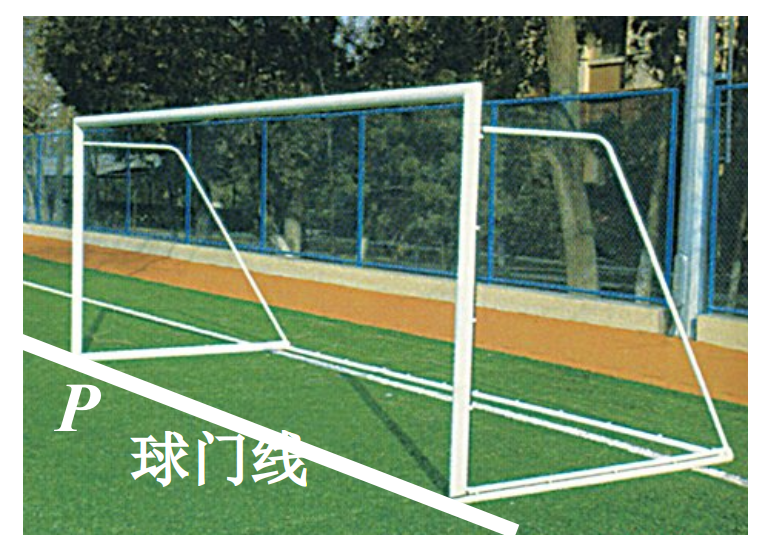
\includegraphics[width=0.3\linewidth]{picture/screenshot003}
\end{figure}

\fourchoices
{足球位移的大小$x = \sqrt { \frac { L ^ { 2 } } { 4 } + s ^ { 2 } }$}
{足球初速度的大小$v _ { 0 } = \sqrt { \frac { g } { 2 h } \left( \frac { L ^ { 2 } } { 4 } + s ^ { 2 } \right) }$}
{足球末速度的大小$v = \sqrt { \frac { g } { 2 h } \left( \frac { L ^ { 2 } } { 4 } + s ^ { 2 } \right) + 4 g h }$}
{足球初速度的方向与球门线夹角的正切值$\tan \theta = \frac { L } { 2 s }$}



\item 
\exwhere{$ 2015 $年上海卷}
如图,战机在斜坡上方进行投弹演练。战机水平匀速飞行,每隔相等时间释放一颗炸弹,第一颗落在$ a $点,第二颗落在$ b $点。斜坡上$ c $、$ d $两点与$ a $、$ b $共线,且$ ab=bc=cd $,不计空气阻力。第三颗炸弹将落在 \xzanswer{A} 
\begin{figure}[h!]
\centering
\includesvg[width=0.23\linewidth]{picture/svg/563}
\end{figure}



\fourchoices
{$ bc $之间}
{$ c $点}
{$ cd $之间}
{$ d $点}


\item 
\exwhere{$ 2016 $年上海卷}
如图,圆弧形凹槽固定在水平地面上,其中$ ABC $是位于竖直平面内以$ O $为圆心的一段圆弧,$ OA $与竖直方向的夹角为$ \alpha $。一小球以速度$ v_{0} $从桌面边缘$ P $水平抛出,恰好从$ A $点沿圆弧的切线方向进入凹槽。小球从$ P $到$ A $的运动时间为\tk{$\frac { v _ { 0 } \tan \alpha } { g }$};直线$ P_{A} $与竖直方向的夹角$ \beta = $ \tk{$\arctan ( 2 \cot \alpha )$}。
\begin{figure}[h!]
\centering
\includesvg[width=0.23\linewidth]{picture/svg/564}
\end{figure}



\item 
\exwhere{$ 2016 $年浙江卷}
在真空环境内探测微粒在重力场中能量的简化装置如图所示。$ P $是一个微粒源,能持续水平向右发射质量相同、初速度不同的微粒。高度为$ h $的探测屏$ AB $竖直放置,离$ P $点的水平距离为$ L $,上端$ A $与$ P $点的高度差也为$ h $。
\begin{enumerate}
\renewcommand{\labelenumi}{\arabic{enumi}.}
% A(\Alph) a(\alph) I(\Roman) i(\roman) 1(\arabic)
%设定全局标号series=example	%引用全局变量resume=example
%[topsep=-0.3em,parsep=-0.3em,itemsep=-0.3em,partopsep=-0.3em]
%可使用leftmargin调整列表环境左边的空白长度 [leftmargin=0em]
\item
若微粒打在探测屏$ AB $的中点,求微粒在空中飞行的时间;
\item 
求能被屏探测到的微粒的初速度范围;
\item 
若打在探测屏$ A $、$ B $两点的微粒的动能相等,求$ L $与$ h $的关系。

\end{enumerate}
\begin{figure}[h!]
\flushright
\includesvg[width=0.25\linewidth]{picture/svg/565}
\end{figure}

\banswer{
\begin{enumerate}
\renewcommand{\labelenumi}{\arabic{enumi}.}
% A(\Alph) a(\alph) I(\Roman) i(\roman) 1(\arabic)
%设定全局标号series=example	%引用全局变量resume=example
%[topsep=-0.3em,parsep=-0.3em,itemsep=-0.3em,partopsep=-0.3em]
%可使用leftmargin调整列表环境左边的空白长度 [leftmargin=0em]
\item
$t = \sqrt { \frac { 3 h } { g } }$
\item 
$L \sqrt { \frac { g } { 4 h } } \leq v \leq L \sqrt { \frac { g } { 2 h } }$
\item 
$L = 2 \sqrt { 2 } h$



\end{enumerate}


}






\end{enumerate}


